\section{GASPI}
% Overview of GASPI/GPI

\subsection{Background} %Is this necessary?
% From where why

\subsection{Fundamentals}
% How it works


\subsection{TODO sections}
GASPI\footnote{http://www.gaspi.de/gaspi/} (Global Programming Address Space Programming Interface) is a PGAS library that focuses on flexibility, performance and fault tolerance. It differs significantly from UPC and UPC++ in that it is not a language extension, but a library much like MPI. The GASPI API specification is best implemented by the GPI-2 library\footnote{http://www.gpi-site.com/}. 

GASPI is shown to be up to an order of magnitude faster than MPI for multi-threaded communication with small messages\cite{Evaluating_GASPI}.The effectiveness and performance of GASPI's one-sided communication is achieved mainly due to the use of remote direct memory accesses (RDMA). Crucially, beyond initial setup, RDMA  does not require cooperation from the remote host to access its memory. The benefits of this direct access enable higher through-puts, lower latencies and little to no  remote CPU involvement.

RDMA is preferably used with hardware features in the form of a supporting network interface card (NIC). This is necessary to manage the data structures in the remote host's memory management unit and handle simple page faults without remote CPU involvement. Similar capabilities can be implemented without a NIC by pinning virtual address mappings at the network programmer level. This is done in order to ensure all pages remain present in memory and crucially at their correct physical locations. However, in case the page pinning is not perfect and a page fault is triggered, a remote host CPU has to be involved to handle the fault - a very significant performance implication. Luckily, in HPC environments, NICs with RDMA are commonplace, for example Infiniband\footnote{https://www.infinibandta.org/} natively supports RDMA.  Therefore, in production the problematic software RDMA is rare. Importantly, however, this software based RDMA enables functionality testing on non-hardware supporting NICs; this is crucial for rapid development and testing. 

%Segments are the GAPSI partitions of the PGAS. From a hierarchical memory model including: GPU, MIC, NUMA, SSD, etc... memory, a segment can provide a virtual heterogeneous memory interface to all (Figure \ref{fig:GPI-2_Diagram}). Therefore, segments can be presented to the programmer as simply a contiguous block of virtual memory, leaving all memory management within the segment is up to the programmer.
GASPI implements segments as the partitions of Partitioned Global Address Space. As depicted in Figure \ref{fig:GPI-2_Diagram}, a segment provides virtual heterogeneous memory interface using different types of memory: GPU's memory, MIC, NUMA, SSD and others. This model allows representing segments to the programmer as a contiguous block of virtual memory and leaves all memory management within the segment up to the programmer. 

\begin{figure}
    \centering
    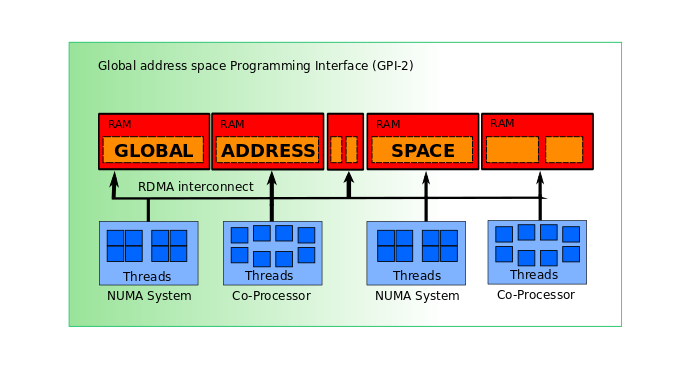
\includegraphics[width=\linewidth]{GPI-2_memory.png}
    \caption{GPI-2 Memory Model \cite{GPI-2_Documentation}}
    \label{fig:GPI-2_Diagram}
\end{figure}

GASPI is built for asynchronous communication; remote memory operations may return with status codes before the remote memory has actually been updated. The only assurance provided on \verb|GASPI_SUCCESS| status code is that the operation has been validated by the networking middleware layer and added to the job queue. Therefore, with no other synchronisation primitives memory status can never be guaranteed without busy waiting.
Thus to ensure validity of operations, some notion of weak synchronisation is provided through notifications. When some remote memory operation is queued, the programmer can also queue a notification that will be delivered once the memory operation is completed. Importantly, memory transaction ordering is never guaranteed, however ordering of notifications and the relationship between memory transaction and notification are always maintained. Thus when a notification is received, the associated transaction is guaranteed to be completed and memory is in a safe state. Such asynchronity coupled with RDMA enables very high data throughput and reduced latency. 

% % This is a singlesentence para, but it lokos good and logical
% The GASPI specification also enforces that all data motion operations are explicit, this provides the same benefit as in UPC++ such that programmers are aware of any overheads or bottlenecks they induce so they can consider other options. 
Similarly to UPC++ all data motion operations in GASPI are explicit as enforced by the specification. This provides the same benefit that programmers making conscious decisions when using computations that may result in significant overheads or bottlenecks. 

A feature special to GASPI that may be out of the scope of this project is fault tolerance. GASPI provides a set of functionality that is designed to enable discovery of process failures. All remote blocking operations include timeouts, thus on remote process failure, all connected peers eventually become aware of this and do not block indefinitely.
In addition, global status codes which can report such information about failures are present. 
%Note, GASPI provides no support in how this fault is dealt with, it is then entirely up to the application to accommodate and redistribute work. 
The way that the fault is handled and work redistributed has to be implemented by the application itself and is not accommodated by GASPI.
